\chapter{Female Doctors}
\label{sec:female}
\section{Extraction Quality Analysis}
\subsection{Manually Create A Page of Female Doctors}


Our final target is to extract female doctors from  Rosenwald Guide. However, female doctors are sparsely distributed in the book, making it hard to evaluate the extraction accuracy and analyse the extraction quality on our core assets, female doctors.

In order to make the evaluation on female doctors possible, we searched the original-ocr text throughout our target years (1887-1906), find the doctor names suffix containing "Mme" or "Mlle" (3 entries per year, 60 in total) and put them into one page, as is shown in Figure~\ref{fig:women_doctors}. We can measure the extraction quality on this page to be aware of the extraction pipeline performance on our most valuable targets.

However, this manually created page also has its limitations. In reality, the female doctors are sparsely distributed, making it different from our concentrated page. In addition, here we only focus on the doctors with "Mlle" and "Mme" suffix, while in the dataset, the doctors' first name could also indicate if it indicates a female doctor. Finally, in our production scenario, we use the original OCR result to aid the image, while in our test here, we use tesseract OCR on our manually created page.
\begin{figure}[htbp]
    \centering
    \includegraphics[width=0.8\linewidth]{Images/2025-page-0101.png}
    \caption{Manually Created Page of Female Doctors}
    \label{fig:women_doctors}
\end{figure}



\clearpage

\subsection{Quantitative Analysis}
Table~\ref{tab:wer_cer_models} reports the extraction results across different models and input settings. Overall, the Gemini~3 model family exhibits substantially lower error rates than the GPT-5 series. However, two observations appear counterintuitive with respect to our production configuration (Gemini~3~Pro with Image+Text input). First, Gemini~3~Flash achieves slightly lower error rates than Gemini~3~Pro. Second, the Image+Text setting combined with Tesseract yields higher error rates than the Image-only input. Although these differences are relatively small, a qualitative inspection of the error cases remains necessary. Given the limited number of female doctors in the corpus, even minor extraction errors may have a disproportionate impact on the final analysis.


\begin{table}[htbp]
\centering
\caption{Word Error Rate (WER) and Character Error Rate (CER) by input source and model}
\label{tab:wer_cer_models}
\renewcommand{\arraystretch}{1.2}
\begin{tabular}{llcc}
\toprule
\textbf{Source} & \textbf{Model} & \textbf{WER} & \textbf{CER}  \\
\midrule
\multirow{4}{*}{Image}
 & Gemini-3 Flash (preview) & 0.0296 & 0.0152   \\
 & Gemini-3 Pro (preview)   & 0.0385 & 0.0205   \\
 & GPT-5 Mini (2025-08-07)  & 0.1627 & 0.1371   \\
 & GPT-5.2 (2025-12-11)     & 0.2544 & 0.2325   \\
\midrule
\multirow{4}{*}{Image + Text Tesseract}
 & Gemini-3 Flash (preview) & 0.0340 & 0.0231   \\
 & Gemini-3 Pro (preview)   & 0.0429 & 0.0258   \\
 & GPT-5 Mini (2025-08-07)  & 0.2988 & 0.2708   \\
 & GPT-5.2 (2025-12-11)     & 0.2559 & 0.2328   \\
\midrule
\multirow{4}{*}{Tesseract}
 & Gemini-3 Flash (preview) & 0.7589 & 0.6387   \\
 & Gemini-3 Pro (preview)   & 0.7825 & 0.6407   \\
 & GPT-5 Mini (2025-08-07)  & 0.8077 & 0.6688   \\
 & GPT-5.2 (2025-12-11)     & 0.7766 & 0.6493   \\
\bottomrule
\end{tabular}
\end{table}



\subsection{Error Case Study}

% Preamble (if not already):
% \usepackage{booktabs}
% \usepackage{xcolor}
% \usepackage{array}
% \newcommand{\diff}[1]{\textcolor{red}{\textbf{#1}}}

\begin{table}[t]
\centering
\footnotesize
\setlength{\tabcolsep}{6pt}
\renewcommand{\arraystretch}{1.15}

\caption{Character-level differences between the reference line and the \texttt{Image+Text} \texttt{Gemini 3 Pro} output (differences highlighted in \diff{red}).}
\label{tab:err_cases_gemini3pro_imgtext_char_stack}

\begin{tabular}{@{}p{0.08\linewidth} >{\ttfamily\raggedright\arraybackslash}p{0.88\linewidth}@{}}
\toprule
\textbf{ID} & \textbf{Text (Reference on top; Model output below)} \\
\midrule

1 &
\textbf{Ref:}~~litauer mlle louise 1892 bienfai\diff{fai}sance 34 l mer v 2 à 4\\
& \textbf{Gemini:}~litauer mlle louise 1892 bienfaisance 34 l mer v 2 à 4\\
\addlinespace

2 &
\textbf{Ref:}~~h\diff{œ}ltzel mlle 1893 boul de courcelles 87 2 à 3\\
& \textbf{Gemini:}~h\diff{oe}ltzel mlle 1893 boul de courcelles 87 2 à 3\\
\addlinespace

3 &
\textbf{Ref:}~~landais mlle 1892 larr\diff{i}be 3 mar merc vend 1 à 4\\
& \textbf{Gemini:}~landais mlle 1892 larr\diff{a}be 3 mar merc vend 1 à 4 \diff{téléphone 59119}\\
\addlinespace

4 &
\textbf{Ref:}~~l\diff{e}der mme c 1893 miromesnil 37 lun mer ven 1 à 3\\
& \textbf{Gemini:}~l\diff{é}der mme c 1893 miromesnil 37 lun mer ven 1 à 3\\
\addlinespace

5 &
\textbf{Ref:}~~chrzanowska mlle de 1897 anc ext des hôp accouch mal des femmes et des enfants mo\diff{n}cey 18 1 à 3\\
& \textbf{Gemini:}~chrzanowska mlle de 1897 anc ext des hôp accouch mal des femmes et des enfants mo\diff{u}cey 18 1 à 3\\
\addlinespace

6 &
\textbf{Ref:}~~bonsignorio mlle oculiste \diff{clin }boul stgermain 61 clin av de châtillon 4 \diff{m j s 10 à midi}\\
& \textbf{Gemini:}~bonsignorio mlle oculiste boul stgermain 61 \diff{m j s 10 à midi} clin av de châtillon 4\\
\addlinespace

7 &
\textbf{Ref:}~~petit mme 1899 damr\diff{e}mont 62 1 à 3\\
& \textbf{Gemini:}~petit mme 1899 damr\diff{é}mont 62 1 à 3\\
\bottomrule
\end{tabular}
\end{table}
After ignoring mismatches that are purely due to control characters (e.g., \texttt{*}), Table~\ref{tab:err_cases_gemini3pro_imgtext_char_stack} summarizes the remaining error cases produced by the Image+Text Gemini~3~Pro configuration. Importantly, none of the observed errors affects gender identification.

In Examples~2,~4,~5, and~7, the output differs from the reference by a single character, typically involving ambiguous glyphs that are difficult to distinguish reliably. In Example~1, the model produces the grammatically correct form \emph{bienfaisance}, whereas the reference contains \emph{bienfaifaisance}, which likely reflects a spelling error in the original record. Example~3 includes an additional field (a telephone number): although this information was not requested, it is extracted correctly and does not interfere with the target fields. Example~6 contains two addresses, which exceeds our predefined schema; the model only omits one title (\emph{Clin}) associated with an address while correctly extracting the remaining information, though in a slightly different order than the reference.

Overall, these errors have no substantive impact on gender recognition. They mainly consist of minor character-level confusions on unclear glyphs and occasional overflow when the record contains information outside the predefined paradigm. We therefore conclude that our extraction pipeline (Image+Text with Gemini~3~Pro Preview) provides reliable performance for female doctor information extraction.

\clearpage
\section{Female Doctors Quantity and Distribution}


First we analyse the count of Mme and Mlle throughout the pages, as is shown in Figure~\ref{fig:dis_mme_mlle}. We can see 3420 out of 4166 files (over 82\%) have no Mme or Mlle at all. The file count decreases nearly exponentially if we increase the total count of Mme and Mlle, illustrating a long tail distribution. This distribution over count of Mme and Mlle shows that the female doctors are sparsely distributed throughout the pages.

\begin{figure}[htbp]
    \centering
    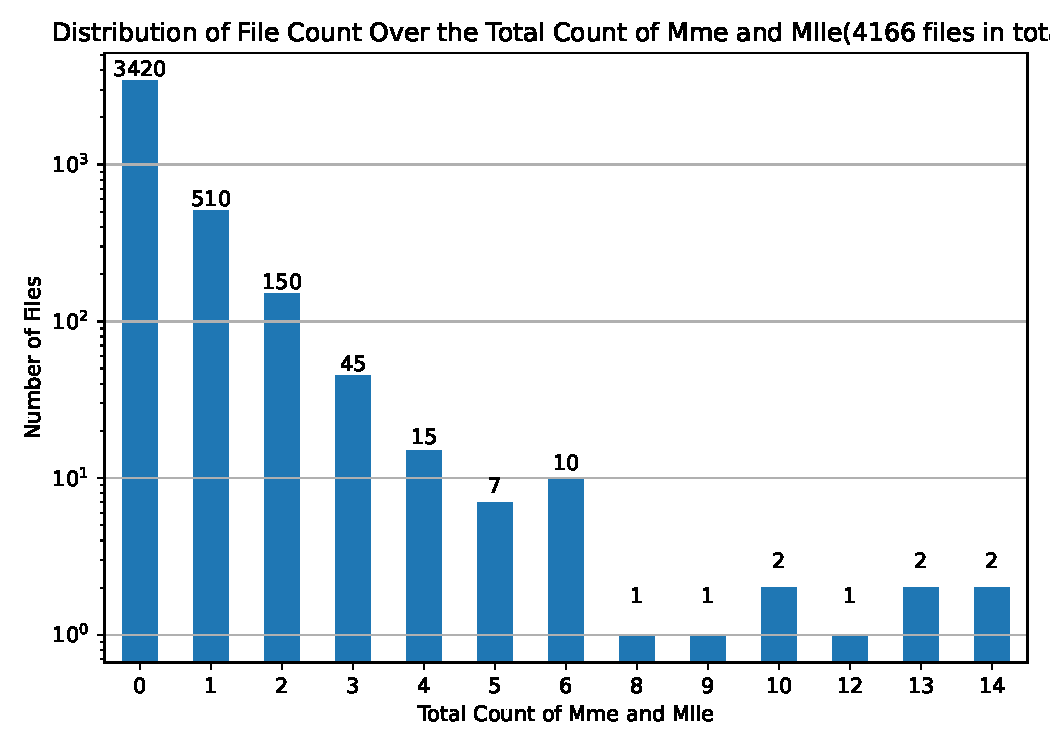
\includegraphics[width=0.52\linewidth]{Images/mme_mlle_total_count_distribution.pdf}
    \caption{Distribution of File Count Over the Total Count of Mme and Mlle}
    \label{fig:dis_mme_mlle}
\end{figure}

Figure~\ref{fig:dis_total_count} shows the count of Mme and Mlle for each page. X axis is sorted by the year and page, in ascending order. For the first page of each year, we add the year label on x axis. We can see that as the years goes more recent, there are more files that have non zero Mme and Mlle count, and the peak value also has an increasing trend. It could be explained as more female doctors are noted in Rosenwald Guide in the later years.

\begin{figure}[htbp]
    \centering
    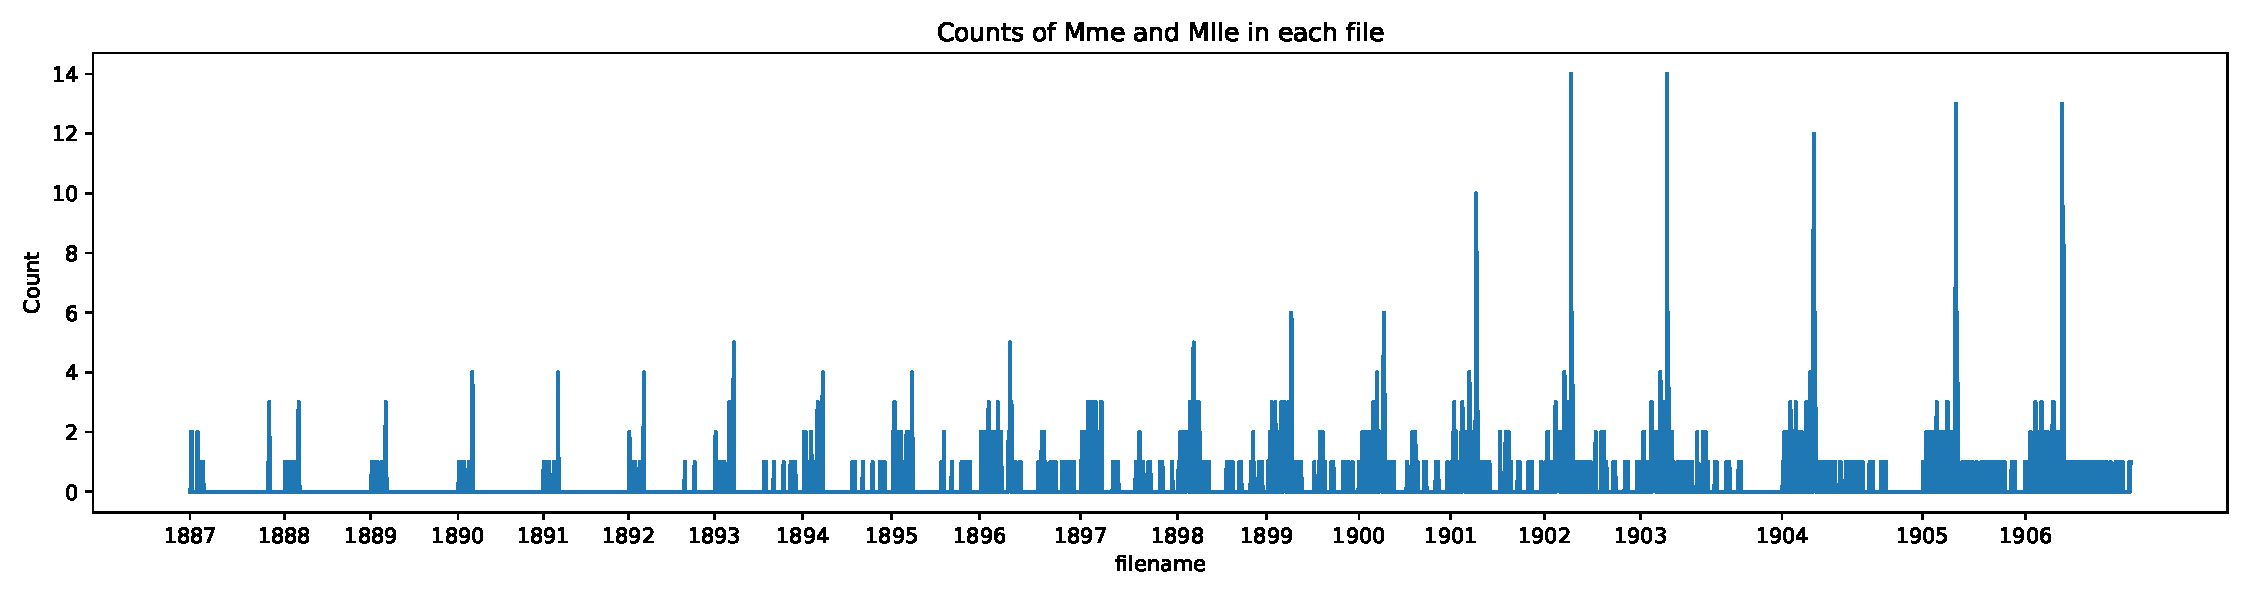
\includegraphics[width=\linewidth]{Images/mme_mlle_counts_per_file_line_plot.pdf}
    \caption{Count of Mme and Mlle for each page}
    \label{fig:dis_total_count}
\end{figure}




Another interesting phenomenon is that the count of Mme and Mlle has a periodic appearance, especially after 1898. The count would quickly come to a peak and then drop. In order to look further into this pattern, we have Figure~\ref{fig:larger5}, showing the Count of Mme and Mlle, sorted descendingly by total Mme and Mlle count.

\begin{figure}[htbp]
    \centering
    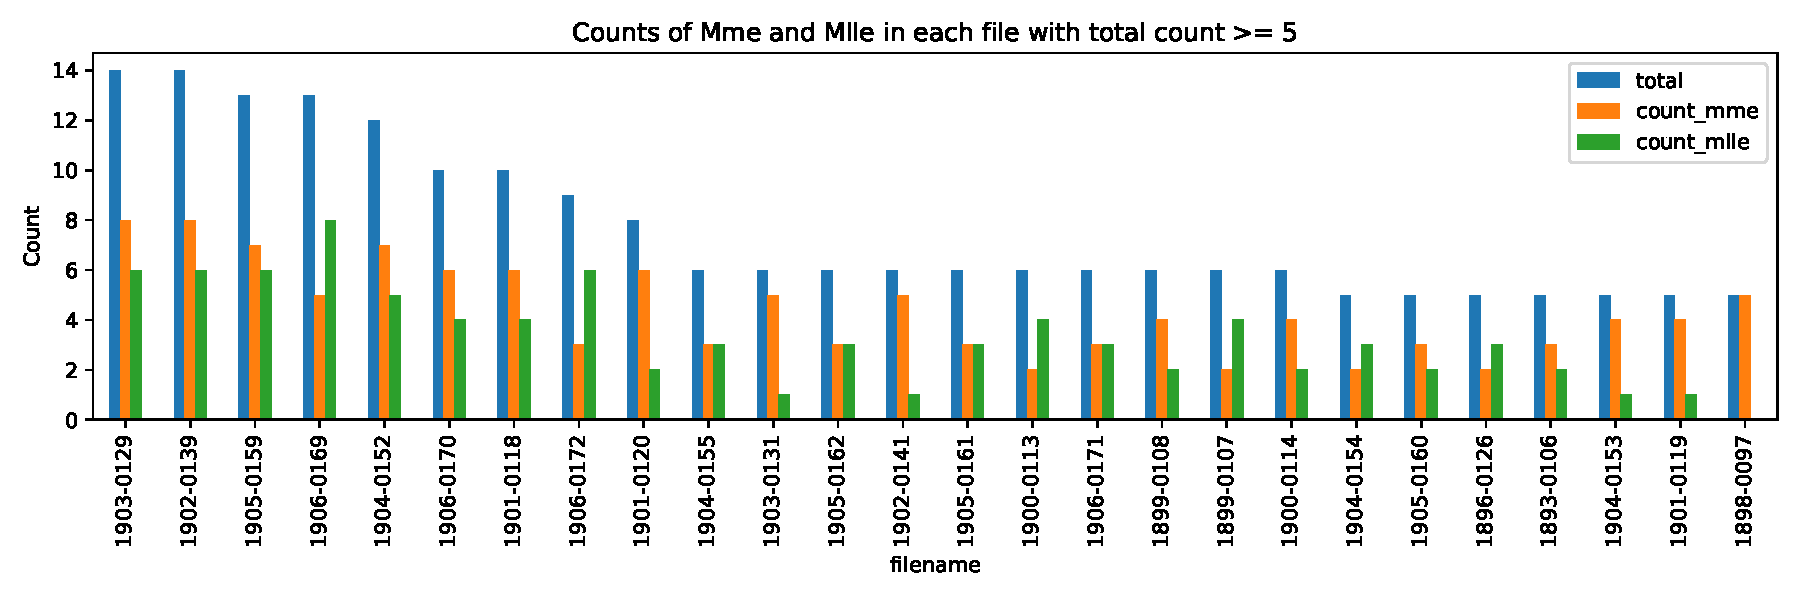
\includegraphics[width=\linewidth]{Images/mme_mlle_counts_per_file_bar_plot.pdf}
    \caption{Counts of Mme and Mlle in each file with total count >= 5}
    \label{fig:larger5}
\end{figure}

\begin{figure}
    \centering
    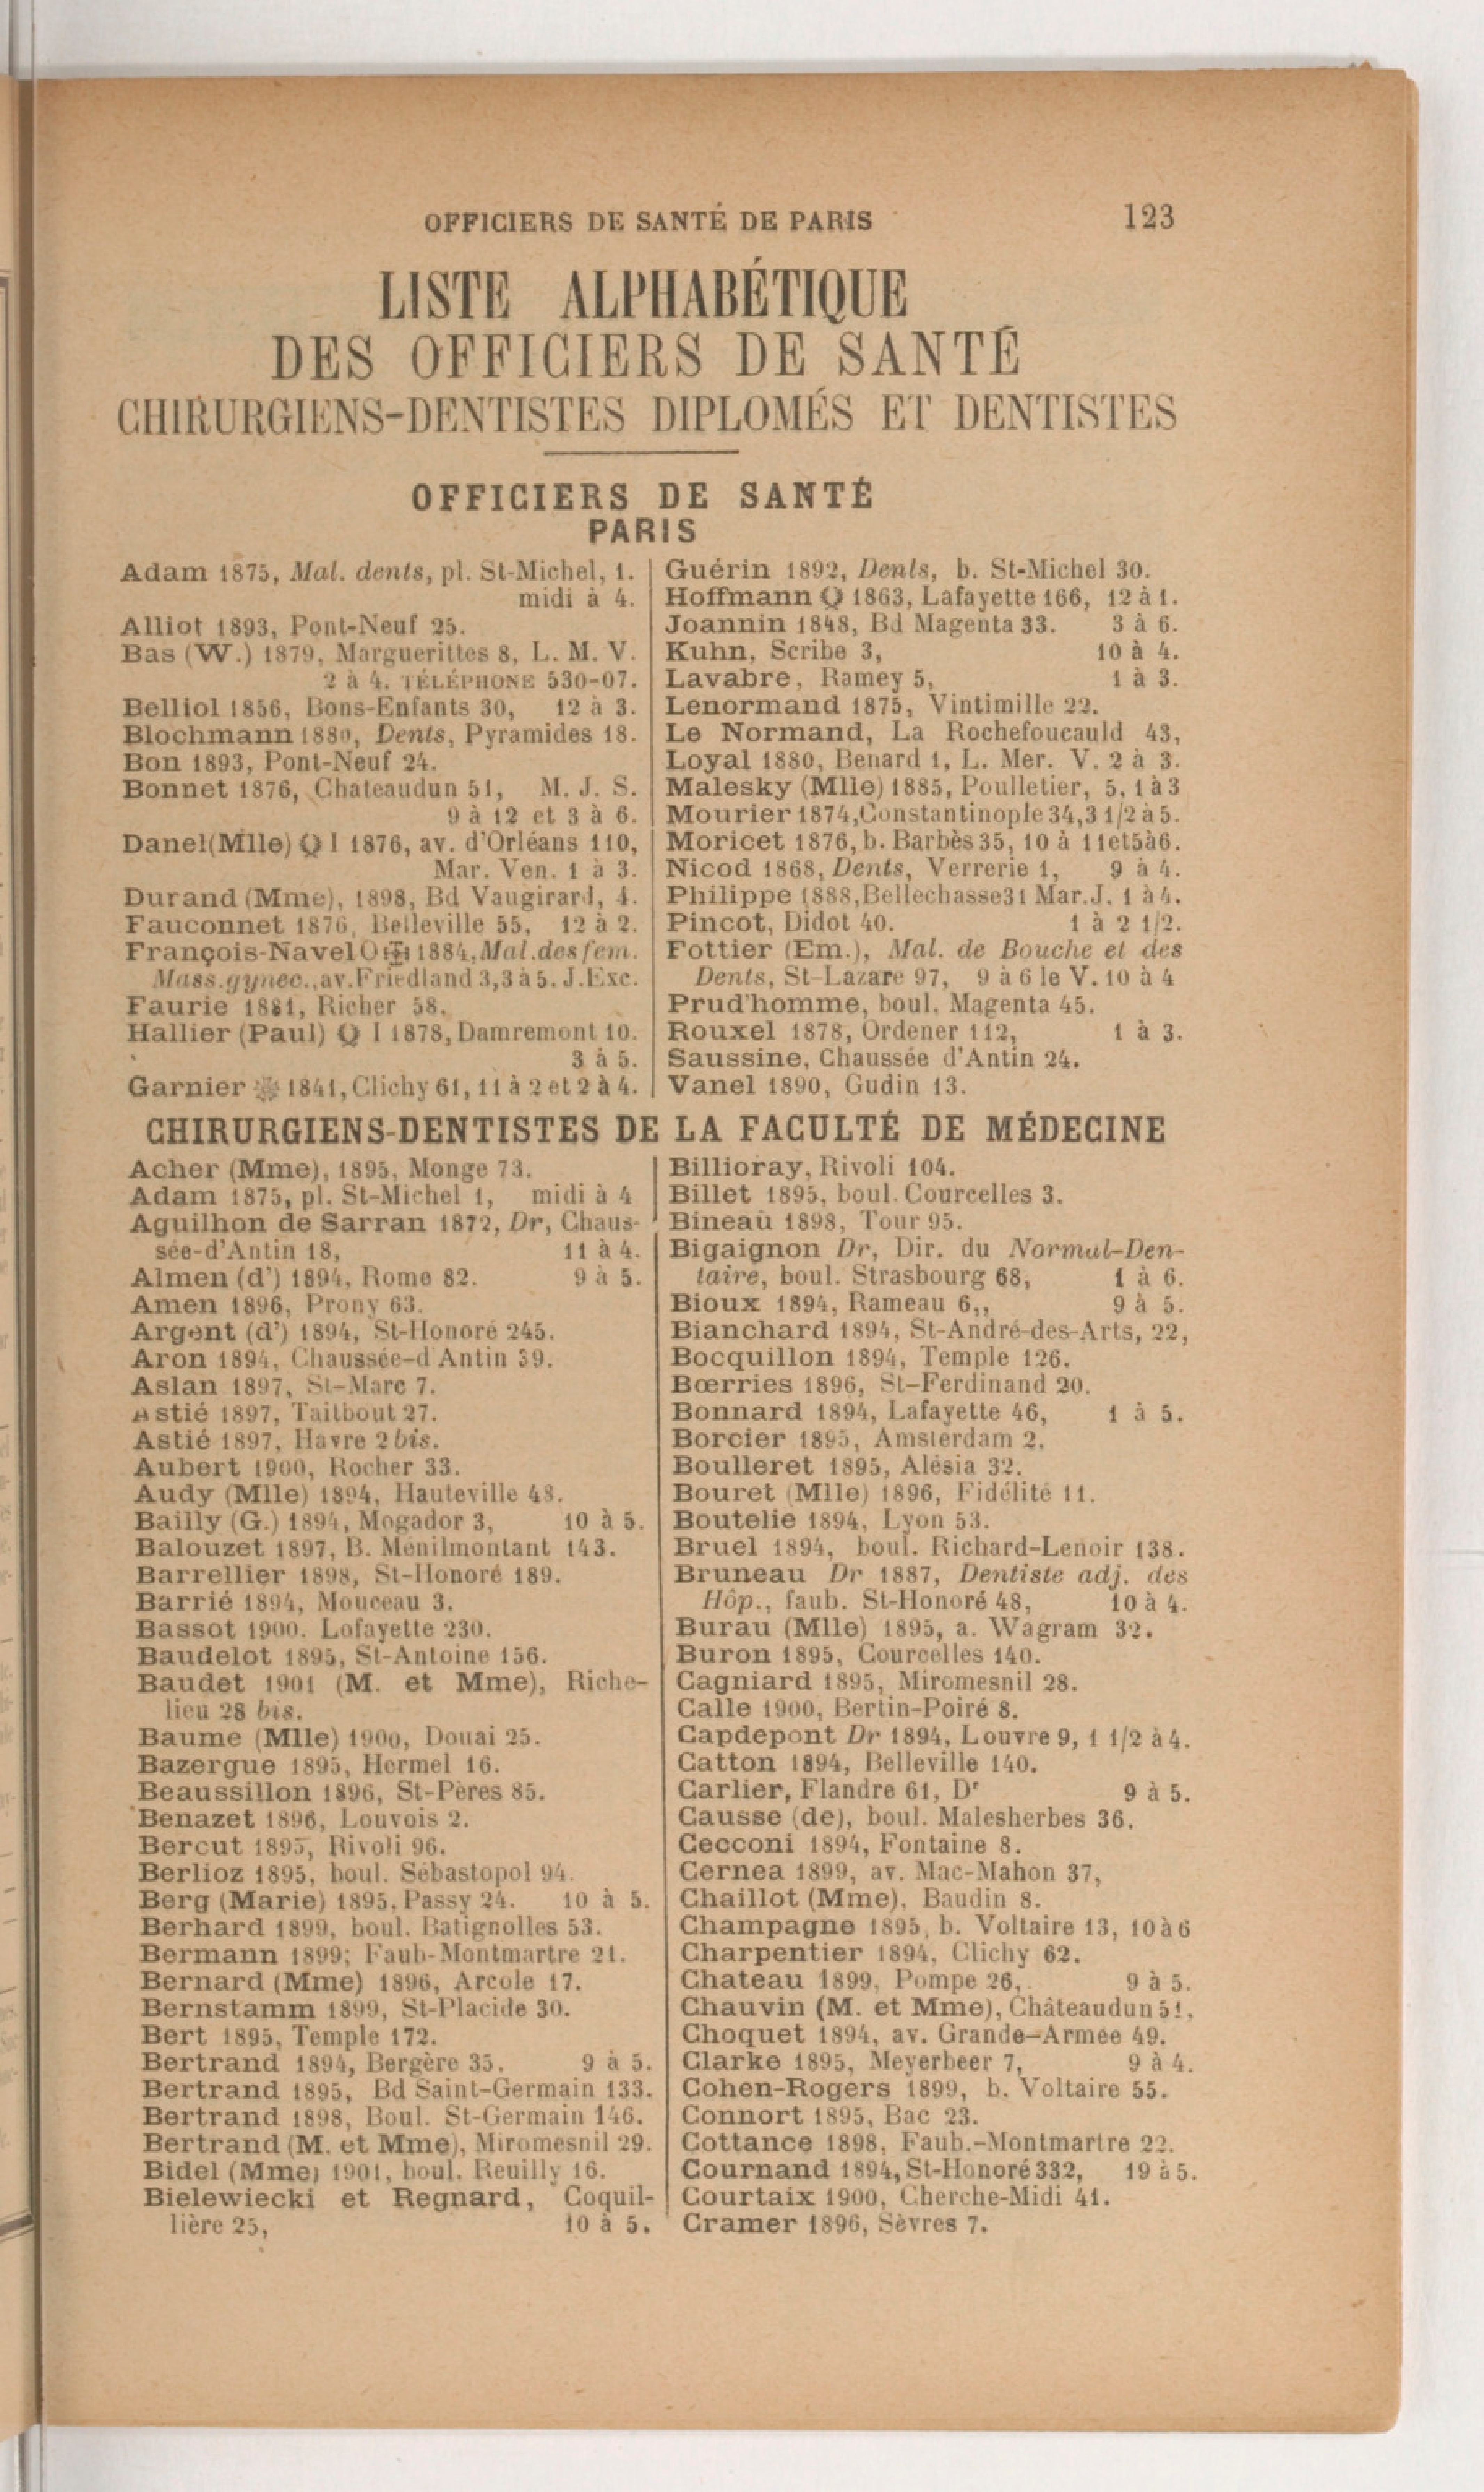
\includegraphics[width=0.9\linewidth]{Images/1902-page-0139.png}
    \caption{1902 Page 139}
    \label{fig:1902_0139_page}
\end{figure}



In the top five peaks, all pages come from the 1902--1906 volumes, and their page numbers cluster within a narrow range (129, 139, 152, 159, 169). Upon inspection, we found that these pages correspond to the opening page of the section \emph{``LISTE ALPHABÉTIQUE DES OFFICIERS DE SANTÉ, CHIRURGIENS-DENTISTES DIPLÔMÉS ET DENTISTES, OFFICIERS DE SANTÉ, PARIS.''} Table~\ref{tab:extrait_notices} presents the female doctors listed on page 139 in the 1902 volume. We then counted how often each name appears across these five pages: 12 of the 14 names occur four or five times, indicating that the top-five peaks in the total counts of \emph{Mme} and \emph{Mlle} are largely driven by the same set of female doctors. These high-frequency entries therefore provide valuable longitudinal samples for analyzing how individual records change over time.


\begin{table}[htbp]
\centering
\small
\setlength{\tabcolsep}{5pt}
\renewcommand{\arraystretch}{1.15}
\begin{tabularx}{\linewidth}{@{}>{\raggedright\arraybackslash}p{3.2cm} >{\centering\arraybackslash}p{2.2cm} >{\centering\arraybackslash}p{1.2cm} >{\raggedright\arraybackslash}p{0.8cm} >{\raggedright\arraybackslash}X >{\raggedright\arraybackslash}p{2.7cm} >{\centering\arraybackslash}p{1.1cm}@{}}
\toprule
\textbf{Nom} & \textbf{\#Appearance} & \textbf{Année} & \textbf{Notes} & \textbf{Adresse} & \textbf{Horaires} & \textbf{Sexe} \\
\midrule
Danel (Mlle) & 5 & 1876 & \makecell[tl]{\(\star\) I} & av.\ d'Orléans 110 & Mar.\ Ven.\ 1 à 3 & Mlle \\
Durand (Mme) & 3 & 1898 &  & Bd Vaugirard, 4 &  & Mme \\
Acher (Mme) & 5 & 1895 &  & Monge 73 &  & Mme \\
Audy (Mlle) & 5 & 1894 &  & Hauteville 43 &  & Mlle \\
Baudet (M.\ et Mme) & 4 & 1901 &  & Richelieu 28 bis &  & Mme \\
Baume (Mlle) & 2 & 1900 &  & Douai 25 &  & Mlle \\
Bernard (Mme) & 5 & 1896 &  & Arcole 17 &  & Mme \\
Bertrand (M.\ et Mme) & 5 &  &  & Miromesnil 29 &  & Mme \\
Bidel (Mme) & 5 & 1901 &  & boul.\ Reuilly 16 &  & Mme \\
Malesky (Mlle) & 5 & 1885 &  & Poulletier, 5 & 1 à 3 & Mlle \\
Bouret (Mlle) & 5 & 1896 &  & Fidélité 11 &  & Mlle \\
Burau (Mlle) & 5 & 1895 &  & a.\ Wagram 32 &  & Mlle \\
Chaillot (Mme) & 4 &  &  & Baudin 8 &  & Mme \\
Chauvin (M.\ et Mme) & 4 &  &  & Châteaudun 51 &  & Mme \\
\bottomrule
\end{tabularx}
\caption{1902 page 139 female doctors (nom, \#appearance, année, notes, adresse, horaires, sexe).}
\label{tab:extrait_notices}
\end{table}

\clearpage
\section{Limitation}

In the brief analysis of this part, we only recognize female doctors by the most significant label "Mme" and "Mlle", while they could also be identified by other information, for example, the first name, if any. However, we do not have enough time to conduct further anlaysis in this work, and it remains a valuable direction for future work.